\scanpage{551}
\mspage{\unsure{281}}

canonical bijection
\[
\tag{33}
\widetilde I \xrightarrow{\sim} V(I)^*
\overset{\mathrm{df}}{=} V(I)\setminus\{0\}
\]
by associating to a partition $I=I'\cup I''$, with
$I',I''$ of cardinality $2$, the \inserted{only} permutation
\unsure{\inserted{(even)}|\deleted{\inserted{(even)}}} of $I$
\deleted{formed of} which \unsure{leaves invariant} $I',I''$ and \unsure{induces|induces} on
each \unsure{its} nontrivial permutation. (The elements
of $\mathfrak{S}_I$ obtained in this way are also the \uline{even}
\uline{permutations} \uline{of order $2$}, \deleted{\unsure{)}} which together with the identity thus form
the subgroup $V(I)$).

We find, if $i\in I$, whence $I\setminus\{i\}$ of
cardinality $3$, \deleted{\unsure{that}} a canonical map
\[
\tag{34}
I\setminus\{i\}\longrightarrow\widetilde I
\]
by associating to $j\in I\setminus\{i\}$ the partition
of $I$ into $\{i,j\}$ and its complement.
This bijection being compatible with the
transport of \unsure{structures|structure}, we conclude
that the corresponding isomorphism
\[
\tag{35}
\mathfrak{S}_{I\setminus\{i\}}\simeq\mathfrak{S}_{\widetilde I}
\]
\deleted{\unsure{which}} is \deleted{\unsure{compat}} also the composite
\[
\tag{36}
\underset{\substack{\text{stabilizer of}\\ i\text{ in }\mathfrak{S}_I}}
{\mathfrak{S}_{I\setminus\{i\}}}
\hookrightarrow\mathfrak{S}_I\longrightarrow\mathfrak{S}_{\widetilde I},
\]
hence the four symmetric subgroups
of index $3$ $\mathfrak{S}_{I\setminus\{i\}}$ of $\mathfrak{S}_I$ $(i\in I)$\unsure{.|,}

\scanpage{552}
are canonically \unsure{isomorphic} to $\mathfrak{S}_{\widetilde I}$
--- hence to one another, \deleted{\unsure{but}} by isomorphisms which
\deleted{\unsure{not}} are \deleted{\unsure{not}} moreover \deleted{\illegible{1}} deduced from the canonical
bijections \deleted{\unsure{equal}}
\[
  (\deleted{\unsure{39}}\inserted{37})\qquad
  I\setminus\{i\}\xrightarrow{\sim}I\setminus\{j\}
  \qquad(i\ne j,\ i,j\in I)
\]
canonical, equal to \deleted{the identity}
\inserted{the \uline{transposition} (not to the identity)} on $I\setminus\{i,j\}$.
\inserted{This bijection is in fact the composite}
\deleted{(Indeed, these bijections \unsure{do not form a}}
\[
  I\setminus\{i\}\xrightarrow{\sim}\widetilde I
  \xrightarrow{\sim}I\setminus\{j\}
  \qquad\text{---}
\]
\deleted{transitive \unsure{system} of isomorphisms.)}
and for variable $i,j$, these isomorphisms form a
transitive system of isomorphisms.

Returning to the action of $\mathfrak{S}_4$ on
$M_{\unsure{0},4}^{!}$, the key to \unsure{understanding}
is given by this:

\uline{Proposition} Consider the subgroup
$V(\deleted{\unsure{4}}\inserted{I})$ of $\mathfrak{S}_{\deleted{\unsure{4}}\inserted{I}}$ formed by $1$ and the even
involutions. Then the action of $V(\deleted{\unsure{4}}\inserted{I})$ on $M_{0,\deleted{\unsure{4}}\inserted{I}}^{!}$
is trivial, \unsure{\&|If} therefore \deleted{$V(I)$} $\mathfrak{S}_I$ acts
on $M_{0,I}^{!}$ through
$\mathfrak{S}_I/V(I)=\mathfrak{S}_{\widetilde I}$.
\figure{\begin{tikzpicture}[x=1cm,y=1cm]
\draw[line width=0.45pt]
  (0,3.45) .. controls (0.00,3.22) and (0.015,3.04) .. (0.045,2.90);
\draw[line width=0.45pt]
  (0.04,1.28) .. controls (0.055,0.83) and (0.055,0.35) .. (0.035,0.10)
  .. controls (0.03,0.04) and (0.015,0.015) .. (0,0);
\end{tikzpicture}}

\margin{\uline{N.B.} $M_{0,I}^{!}$ is defined in \unsure{terms} of $I$, for every set\unsure{.} $I$ of cardinality\unsure{.} $\geq 3$, as $M_{0,n}^{!}$}

\uline{Corollary} Let $i\in I$, then the action
of $\mathfrak{S}_{I\setminus\{i\}}\subset\mathfrak{S}_I$ on $M_{0,I}^{!}$ is deduced
from that of $\mathfrak{S}_{\widetilde I}$ via the canonical isomorphism $\mathfrak{S}_{I\setminus\{i\}}\xrightarrow{\sim}\mathfrak{S}_{\widetilde I}$

\scanpage{553}
\mspage{28\unsure{0|1}bis}
\deleted{\unsure{of}} of the subgroups
\[
 (31)\qquad \mathfrak{S}_3\times\mathfrak{S}_{n-3}\subset\mathfrak{S}_n
\]
of $\mathfrak{S}_n$ on $M_{0,n}^{!}$, and not of \unsure{that|those} of
the whole of $\mathfrak{S}_n$. In the case $n=4$,
the operation of $\Gamma'_2=\mathrm{Sl}(2,\mathbb{F}_2)\simeq\mathfrak{S}_3$ on
$M_{0,4}^{!}$ which interests us, is the one which
corresponds to the subgroup $\mathfrak{S}_{\unsure{1}}\times\mathfrak{S}_3\subset\mathfrak{S}_4$,
which fixes the first element (\unsure{corresponding} to
the zero section of an elliptic curve
--- \deleted{\unsure{which}} and which permutes the three \unsure{following ones}
\unsure{corresponding} to the three elements of order $2$
of a geometric elliptic curve in \unsure{characteristic} $\ne 2$, which
are the three other \unsure{poin\textsuperscript{t}s} fixed by
$x\mapsto -x$, whereas the \unsure{naive|naive} operation of
$\mathfrak{S}_3$ on $U_{0,3}$ corresponds to the subgroup
$\mathfrak{S}_3\times\mathfrak{S}_1$ of $\mathfrak{S}_4$, which fixes the first three
elements. A little question of \unsure{scheme-theoretic}
gymnastics (\unsure{independent|independent} now of the
geometry of elliptic curves, but
a matter of projective geometry of dimension $1$):
how to pass from one of these \deleted{\unsure{representations}}\inserted{actions of}
$\mathfrak{S}_3$ to the other? We feel like proving that
they are the same!

\scanpage{554}
Let us note that if $I$ is a set with $4$
elements, then associated to it is a
three-element set of ``partitions of
type $(2,2)$'' $P_{2,2}(I)=\widetilde I$, and the homomorphism
\[
 (32)\qquad
 \diagram{\begin{tikzcd}[ampersand replacement=\&, row sep=small,column sep=large]
 \mathfrak{S}_I \arrow[r] \arrow[d,phantom,"\simeq"{rotate=90}]
   \& \mathfrak{S}_{\widetilde I} \arrow[d,phantom,"\simeq"{rotate=90}] \\
 \mathfrak{S}_4 \& \mathfrak{S}_3
 \end{tikzcd}}
\]
is surjective --- its kernel is a subgroup
isomorphic (\unsure{not} canonical\textsuperscript{ly}) to $\mathbb{F}_2\times\mathbb{F}_2$ --- hence a
commutative group \inserted{$V(I)$} killed by $2$, i.e. a
vector space over $\mathbb{F}_2$, and as such of dimension $2$.

In fact, $V(I)$ \unsure{operating} on $I$ makes $I$
a $V(I)$ torsor --- so $I$ is canonically equipped
with a structure \unsure{of|of} an affine \deleted{\unsure{space}}\inserted{plane} over $\mathbb{F}_2$,
and $V(I)\subset\mathfrak{S}_I$ is its group of
translations, $\mathfrak{S}_I$ \unsure{being interpreted|is interpreted} as the
group of affine automorphisms of $I$ (\uline{\unsure{every}} permutation
of $I$ is affine --- there \deleted{\unsure{not}} is on the set
$I$ $1$ and only $1$ affine plane structure over
$\mathbb{F}_2$), and $\mathfrak{S}_{\widetilde I}$ as the group $\mathrm{Aut}(V(I))$
--- which suggests interpreting $\widetilde I$ as
the set of the three nonzero elements of $V(I)$, and
indeed, we observe that \deleted{\unsure{the}} we have a

\scanpage{555}
\mspage{282}

coming from $I\setminus\{i\}\xrightarrow{\sim}\widetilde I$.

In particular, for $I=[1,2,3,4]$, to
compare the action of $\mathfrak{S}_{\{1,2,3\}}$ and of
$\mathfrak{S}_{\{2,3,4\}}$ on $M_{0,4}^{!}\simeq U_{0,3}$ --- where the first
is the standard action of $\mathfrak{S}_3$ on $U_{0,3}$,
the second that of $\mathfrak{S}_3$ on $M_{1,1}[2]'$,
we use the isomorphism
\[
\tag{38}
\mathfrak{S}_{\{1,2,3\}}\simeq\mathfrak{S}_{\{2,3,4\}}
\]
made explicit in (37), corresponding to the
bijection
\[
1\mapsto4,\quad 2\mapsto3,\quad 3\mapsto2
\]
of the index \unsure{sets}, which therefore corresponds
to the \unsure{automorphism}
\[
\tag{39}
\operatorname{int}(\sigma_1):\mathfrak{S}_3\longrightarrow\mathfrak{S}_3
\]
now identifying the two index
sets $[1,2,3]$, $[2,3,4]$ with $\{0,1,\infty\}$,
and denoting by $\sigma_i\in\mathfrak{S}_{\{0,1,\infty\}}$
\inserted{(for $i\in\{0,1,\infty\}$)} the
transposition of the elements $\ne i$. Thus

\uline{Corollary} The canonical isomorphism
\[
U_{0,3}\xrightarrow{\overset{\varphi}{\sim}}M_{1,1}[2]'
\qquad (\text{over }\mathbb Z[1/2]),
\]
when we let $\mathfrak{S}_3=\mathfrak{S}_{\{0,1,\infty\}}$ operate on
both sides, is compatible
with its operations, \uline{via} the \unsure{automorphism} $\operatorname{int}(\unsure{\sigma_1|\sigma_i})$, i.e.

\scanpage{556}

\[
\tag{40}
\varphi(u.x)=(\unsure{\sigma_1|\sigma_i}\,u\,\unsure{\sigma_1^{-1}|\sigma_i^{-1}})\varphi(x)
\]

We must all the same prove proposition 4,
which \unsure{is equivalent} of course to this

\uline{Corollary} Let $X$ be a relative projective line
over \unsure{scheme} $S$, $I$ \unsure{set} with four elements,
$(\deleted{\unsure{\sigma_i}}s_i)_{i\in I}$ a family of \unsure{mutually|mutually}
disjoint sections, and $\sigma$ an even \deleted{\unsure{transposition}}\inserted{\unsure{involution}} of
$I$ (corresponding to a partition $I=\{i_1,i_2\}\cup\{i_3,i_4\}$
by $\sigma i_1=i_2$, $\sigma i_2=i_1$, $\sigma i_3=i_4$, $\sigma i_4=i_3$). Then $\exists$
\unsure{automorphism} (obviously unique) $u$ of $X$,
such that $u\circ s_i=s_{\sigma i}$.

\uline{Proof} We may suppose $X=\mathbb P^1_S$, $\unsure{s_1|s_{i_1}}=0$, $s_{i_2}=\infty$, hence
$\unsure{s_{i_2}|s_{i_4}},s_{i_3}$ identify with sections of
$\underline{\mathcal O}_S^*$, we will take \deleted{\illegible{1}} $u$ defined by
\[
u(z)=\lambda/\unsure{z|Z}\qquad\lambda\in\Gamma(S,\mathcal O_S^*)
\]
which exchanges $0$ and $\infty$, and the condition
for exchanging $s_2,s_3$ \unsure{will be|is written} $\lambda/s_3=s_4$, $\lambda/s_4=s_3$
i.e. $\lambda=s_3s_4$ (\uline{N.B.} it \unsure{sufficed|would suffice} that
$(s_1,s_2,s_3)$ and $(s_1,\unsure{s_2|s_1},s_4)$ \unsure{are|be} mutually disjoint ---
no need for $s_3,s_4$ to be mutually
disjoint $\ldots$)

\scanpage{557}
\mspage{283}

Let us again work over $\mathbb Q$ (to fix
ideas), and consider the fundamental groups
of the modular multiplicities $M_{1,1}$, $M_{1,1}'$.
We start from
\[
\tag{41}
\left\{
\diagram{\begin{tikzcd}[ampersand replacement=\&, column sep=small,row sep=large]
M_{1,1}\arrow[d]\arrow[r,phantom,"\simeq" description]
  \& (M_{1,1}[n],\Gamma_n)\arrow[d]
  \& (n\geq3) \\
M_{1,1}'\arrow[r,phantom,"\simeq" description]
  \& (M_{1,1}[n],\underset{\substack{\Vert\\\Gamma_n/\pm1}}{\Gamma_n'})
  \& {\begin{gathered}(n\geq2\unsure{)},\text{ replacing}\\
      \text{for }n=2\quad M_{1,1}[2]\text{ by}\\
      M_{1,1}[2]')\end{gathered}}
\end{tikzcd}}
\right.
\]
which \unsure{gives|give} \unsure{isomorphisms} of outer groups
\[
\tag{42}
\diagram{\begin{tikzcd}[ampersand replacement=\&, column sep=small,row sep=large]
\deleted{\unsure{\{}}\pi_1(M_{1,1})\arrow[d]\arrow[r,phantom,"\simeq" description]
  \& \pi_1(M_{1,1}[n],\Gamma_n)\arrow[d]
  \& (n\geq3) \\
\pi_1(M_{1,1}')\arrow[r,phantom,"\simeq" description]
  \& \pi_1(M_{1,1}[n],\Gamma_n')
  \& {\begin{gathered}(n\geq2\unsure{)},\text{ with}\\
      \text{same grain of salt}\\
      \text{for }n=2)\end{gathered}}
\end{tikzcd}}
\]

since $M_{1,1}[n]$ is connected (even if it is not
geometrically connected), we find
\margin{this is Kronecker's theorem on the irreducibility of the cyclotomic equation}
\[
\tag{43}
\left\{
\diagram{\begin{tikzcd}[ampersand replacement=\&, column sep=small,row sep=large]
1\arrow[r,dash]
  \& \pi_1(M_{1,1}[n])\arrow[r]\arrow[d,"\sim"]
  \& \pi_1(M_{1,1}\deleted{\unsure{[n]}})\arrow[r,dash]\arrow[d]
  \& \Gamma_n\arrow[r]\arrow[d]
  \& 1 \\
1\arrow[r,dash]
  \& \pi_1(M_{1,1}[n])\arrow[r]
  \& \pi_1(M_{1,1}\deleted{\unsure{[n]}}')\arrow[r,dash]
  \& \Gamma_n'\arrow[r,dash]
  \& 1
\end{tikzcd}}
\right.
\]
which allows us to \unsure{reconstruct|reconstruct} $\pi_1(M_{1,1})$, as
an extension of $\Gamma_n$, when we
\unsure{know|know} $\pi_1(M_{1,1}')$ as an extension of
$\Gamma_n'$, by inverse image via $\Gamma_n\to\Gamma_n'$. We
find \deleted{\illegible{2}}\inserted{as} is only right

\figure{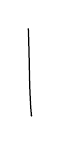
\begin{tikzpicture}[x=1cm,y=1cm]
\draw[line width=0.45pt]
  (0,0.63) .. controls (0.015,0.30) and (0.01,-0.18) .. (0.04,-0.48);
\fill (0.04,-0.48) circle[radius=0.012cm];
\end{tikzpicture}}
\uline{Proposition} $\pi_1(M_{1,1})$ is a central extension
of $\pi_1(M_{1,1}')$ by $\{\pm1\}$.

On the other hand, we have the exact sequences,
\deleted{\illegible{5}}
of homotopy over $\operatorname{Spec}\mathbb Q$

\scanpage{558}

\diagram{(44)\quad
\begin{tikzcd}[ampersand replacement=\&, column sep=small]
1 \arrow[r,no head] \&
\pi_1(\overline{M}_{1,1})\inserted{{}=\widehat{\mathcal T}_{1,1}^{+}} \arrow[r] \arrow[d] \&
\pi_1(M_{1,1})\inserted{{}=\mathcal E_{1,1}=N_{1,1}} \arrow[r] \arrow[d] \&
\mathbb{\Gamma}_{\mathbb Q} \arrow[r,no head] \arrow[d] \& 1 \\
1 \arrow[r,no head] \& \pi_1(\overline{M'_{1,1}}) \arrow[r,no head] \&
\pi_1(M'_{1,1}) \arrow[r,no head] \& \mathbb{\Gamma}_{\mathbb Q} \arrow[r,no head] \& 1
\end{tikzcd}}

and the transcendental theory provides
canonical \inserted{outer} isomorphisms

\diagram{(45)\quad
$\left\{
\begin{tikzcd}[ampersand replacement=\&, column sep=large,row sep=large]
\pi_1(\overline{M}_{1,1}) \arrow[d] \arrow[r,phantom,"\simeq" description]
 \& \mathrm{Sl}(2,\mathbb Z)^{\wedge} \arrow[d] \\
\pi_1(\overline{M'_{1,1}}) \arrow[r,phantom,"\simeq" description]
 \& \mathrm{Sl}(2,\mathbb Z)'^{\wedge}=\mathrm{Sl}(2,\mathbb Z)^{\wedge}/\mathord{\pm}1,
\end{tikzcd}\right.$}

\margin{Careful not to confuse $\mathrm{Sl}(2,\mathbb Z)^{\wedge}$ with $\mathrm{Sl}(2,\widehat{\mathbb Z})$ !!!}

\deleted{\unsure{whence} \illegible{1} fact that the sequence}

We have \unsure{the} following essential
compatibility between (43) (44) (45): the \unsure{commutativity|compatibility} of

\diagram{(46)\quad
\begin{tikzcd}[ampersand replacement=\&,column sep=1.8em,row sep=1.25em]
1\arrow[r]
\& \pi_1(\overline M_{1,1})\arrow[r]
   \arrow[d,phantom,"\simeq"{description,rotate=90}]
\& \pi_1(M_{1,1})\arrow[r]\arrow[dd]
   \arrow[r,phantom,"{\deleted{\unsure{\longrightarrow\Gamma_n=\mathrm{Gl}(2,\mathbb Z_n)}}}"{description,yshift=-3.8ex,fill=none,inner sep=0pt}]
\& \mathbb{\Gamma}_{\mathbb Q}\arrow[r]
   \arrow[dd,"{\substack{\chi_n\ \text{cyclotomic}\\\text{character}}}"{right}]
\& 1\\
\& \mathrm{Sl}(2,\mathbb Z)^{\wedge}\arrow[d,"\text{surjective}"{right}]
\& \& \& \\
1\arrow[r]
\& \mathrm{Sl}(2,\mathbb Z/n\mathbb Z)\arrow[r,hook]
\& \Gamma_n=\mathrm{Gl}(2,\mathbb Z/n\mathbb Z)\arrow[r,"\det"]
\& (\mathbb Z/n\mathbb Z)^*\arrow[r]
\& 1
\end{tikzcd}}

Passing to the limit over $n$, this gives
a commutative diagram

\diagram{(47)\quad
\begin{tikzcd}[ampersand replacement=\&, column sep=small]
1 \arrow[r,no head] \&
\bigl(\pi_1(\overline{M}_{1,1})\simeq\mathrm{Sl}(2,\mathbb Z)^{\wedge}\bigr) \arrow[r] \arrow[d,"\text{surjective}"'] \&
\pi_1(M_{1,1}) \arrow[r] \arrow[d] \&
\mathbb{\Gamma}_{\mathbb Q} \arrow[r,no head] \arrow[d,"\chi"] \& 1 \\
1 \arrow[r,no head] \& \mathrm{Sl}(2,\widehat{\mathbb Z}) \arrow[r,hook] \&
\mathrm{Gl}(2,\widehat{\mathbb Z}) \arrow[r] \&
\widehat{\mathbb Z}^{*} \arrow[r] \& 1
\end{tikzcd}}

-- diagram to which we will return.

\scanpage{559}
\mspage{284}

For now I am going to exploit the \inserted{second} isomorphism (42), $n=2$:
\[
(48)\qquad
\begin{aligned}
\pi_1(M_{1,1}')\inserted{{}\simeq\deleted{\unsure{\mathcal T_{1,1}^{+}}}N_{1,1}'}
&\simeq\pi_1(M_{1,1}[2]',\Gamma_2=\mathfrak S_3)\\
&\simeq\pi_1(U_{0,3},\mathfrak S_3),
\end{aligned}
\]
where the last isomorphism corresponds to
the isomorphism \inserted{$\operatorname{int}(\sigma_1):$} $\mathfrak S_3\simeq\mathfrak S_3$ made explicit in (40).

We do indeed find, as foreseen in the
preceding \S\ -- and in an entirely
conceptual way, the isomorphism \deleted{of sequences}
\deleted{exact} of extensions

\deleted{(\unsure{49})\quad $\pi_1(M_{1,1}')\simeq\unsure{\widehat{\mathcal T}_{1,1}^{+\,\prime}}\simeq$}

\diagram{(49)\quad
\begin{tikzcd}[ampersand replacement=\&, column sep=small]
1 \arrow[r] \&
\pi_1(\overline{M_{1,1}'})\inserted{{}=\unsure{\widehat{\mathcal T}_{1,1}^{+\,\prime}}\simeq\mathrm{Sl}(2,\mathbb Z)^{\wedge}} \arrow[r] \arrow[d,"\sim"'] \&
\pi_1(M_{1,1}')\inserted{{}\simeq N_{1,1}'} \arrow[r] \arrow[d,"\sim"'] \&
\mathbb{\Gamma}_{\mathbb Q} \arrow[r,no head] \arrow[d,equal] \& 1 \\
1 \arrow[r] \& \pi_1(\overline U_{0,3};\mathfrak S_3) \arrow[r] \arrow[d,"\simeq" description,phantom] \&
\pi_1(U_{0,3},\mathfrak S_3) \arrow[r,no head] \arrow[d,"\simeq" description,phantom] \&
\mathbb{\Gamma}_{\mathbb Q} \arrow[r,no head] \& 1 \\
\& \widehat\Pi_{0,3}' \& \mathcal E_{0,3}'
\end{tikzcd}}

Besides, taking up these reflections again in the
transcendental context, we see that
this isomorphism

\diagram{(50)\quad
\begin{tikzcd}[ampersand replacement=\&, column sep=large]
\widehat\Pi_{0,3}' \arrow[r,"\sim"] \arrow[d,equal] \&
\pi_1(\overline{M_{1,1}'}) \arrow[d,"\simeq" description,phantom] \\
\widehat\Pi_{0,3}/\{\ell_1^2,\ell_\infty^3\} \&
\mathrm{Sl}(2,\mathbb Z)'^{\wedge}=\mathrm{Sl}(2,\mathbb Z)^{\wedge}/\mathord{\pm}1
\end{tikzcd}}

is associated with an isomorphism
\diagram{(51)\quad
$\boxed{\begin{array}{ccc}
\Pi_{0,3}'&\xrightarrow{\sim}&\mathrm{Sl}(2,\mathbb Z)'\simeq\mathrm{Sl}(2,\mathbb Z)/\mathord{\pm}1\\
\Vert&&\\
\Pi_{0,3}/\{\ell_1^{\unsure{2}},\ell_\infty^3\}&&
\end{array}}$}

\scanpage{560}

deduced from the isomorphism of complex analytic
multiplicities
\[
(52)\qquad M_{1,1}^{\mathrm{an}\,\prime}\simeq
(U_{0,3}^{\inserted{\mathrm{an}}}\deleted{\unsure{(\mathbb C)}},\mathfrak S_3)
\]

We should all the same make
the homomorphism (51) explicit -- which is defined only
modulo inner automorphisms, a priori,
by explicit formulas -- whereas
its definition here comes out in a purely conceptual, ``geometric'' way (in the sense
of relative algebraic geometry, of
rational and elliptic curves over
arbitrary analytic spaces). This is
a key calculation, \inserted{surely instructive,} which should not
present any particular \uline{difficulty}\ldots

I have somewhat dropped \inserted{along the way} in all
this the ``coarse'' modular scheme $\widetilde M_{1,1}$,
after having asserted that it is $\simeq\mathbb E_{\mathbb Z}^{1}$, and
that there are two marked sections,
whose \deleted{points} values in characteristic $0$ correspond
\deleted{\unsure{to the}} \inserted{two} isomorphism classes of
\unsure{anharmonic} elliptic curves. In terms of the isomorphism
